\newpage
\subsubsection{Key Storage} \label{section:counter-replace-encryption-key}
In order to use encrypted content, a decryption key is needed.

\subsubsection{Key Storage - Online and Caching} \label{section:counter-replace-encryption-key-online}
The first approach to handle the encryption key is to store it on a server and provide it to the application (see figure~\ref{fig:encryptionKeyServer}).
This works similar to the license verification, but affects the whole content.
\newline
The key can either be retrieved from the server for each decryption action or it can be cached on the device.
Caching should be favored, since getting the key for each action not only requires permanent online connection, but slows down the application and generates additional traffic.
\newline
In the caching scenario, on \textit{decrypt()} call, the application tries to retrieve a cached cryptographic key, which it may have received and stored earlier.
In case a cached key is available, the application starts to decrypt the content.
Otherwise the key is requested from the server.
The server does a verification of the user and when the check is successful, the decryption key is provided.
\newline
\begin{figure}[h]
    \centering
    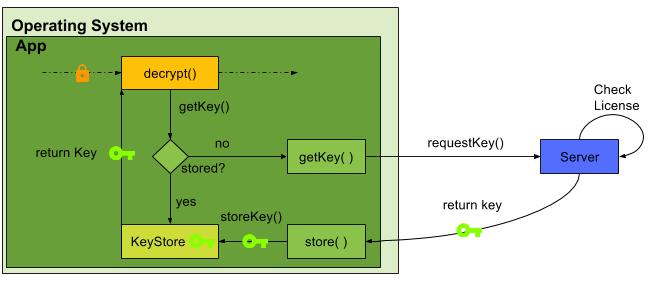
\includegraphics[width=1\textwidth]{data/encryptionKeyServer.png}
    \caption{Retrieving the key after successful identification from the server and store it local on device}
    \label{fig:encryptionKeyServer}
\end{figure}
\newline
A cached key can be stolen \cite{memoryDump} and the encryption cracked this way.
A key needs to be protected against theft and should be changed periodically, e.g. when updating the version of the application.
When running a content server, the key can be user or device specific and changed more often.

\subsubsection{Key Storage - Secure Element} \label{section:counter-replace-encryption-key-local}
A sophisticated way to provide and store a cryptographic key, is the use of a \gls{se}.
\newline
A \gls{se} is a tamper-resistant platform which can be used to securely host simple applications and cryptographic keys \cite{seDefinition}.
There are different form factors for \gls{se}s, i.e. Universal Integrated Circuit Card (UICC), embedded \gls{se} and microSD \cite{seDefinition}.
For Android, the microSD is the form factor of choice.
It can be either mounted in the microSD card slot or on the USB interface by using an adapter.
Using the USB interface requires the Android device to support \gls{otg} \cite{usbOtg}.
The \gls{se} is accessed over reads and writes to its filesystem.
Since the \gls{se} has to be small to fit the size of a microSD card and is powered by the host system, its hardware capabilities are constrained.
The result is a performance as low as 25MHz as compared to the GHz of the system's CPU.
This does not allow complex computations on the \gls{se} \cite{stSe}.
For this reason, the usage of the \gls{se} is restricted to simple tasks, like decryption.
The decryption key is either provided up front on the \gls{se} or the \gls{se} implements a secure mechanism to get the key.
In any case, it needs to relate to the key used for encryption.
The management of this relationship can be quite complex, e.g. involving a certification authority.
The advantage of an \gls{se} is that its functionality is outside of the Android application and thus cannot be manipulated by \gls{luckypatcherg}.
\newline
An abstract presentation for a \gls{se} implementing a decryption method can be seen in figure~\ref{fig:encryptionKeySmart}.
\newline
\begin{figure}[h]
    \centering
    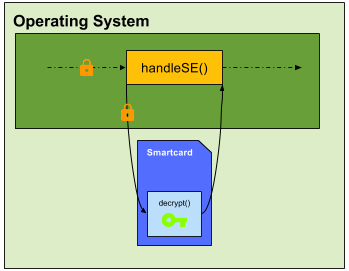
\includegraphics[width=0.5\textwidth]{data/encryptionKeySmart.png}
    \caption{Decryption by using a smartcard}
    \label{fig:encryptionKeySmart}
\end{figure}
\newpage
At the moment, there are some problems with the integration of \gls{se}s.
\begin{itemize}
  \item it invovles extra hardware
  \item not all devices have a spare microSD card slot or support \gls{otg}
  \item no standardized communication protocols for the \gls{se} across manufacturers
\end{itemize}
The first problem is that this requires extra hardware and the hardware has to be around to use the functionality.
\newline
The second problem is the \gls{se} mounted on an external interface for devices without an microSD card slot.
It is no convenient solution and an easy target of an attack.
\newline
The third problem is that some devices without microSD card do not support \gls{otg}.
For example, the Nexus 7 (2012) and the Nexus 6P neither have the capability to use a microSD card.
While the Nexus 7 (2012) is supposed to have \gls{otg}, it does not work with the tested \gls{se}, while the Nexus 6P does not support \gls{otg} at all.
\newline
The fourth problem is the lack of standards.
An application written to use \gls{se} would need to have variants for each device type and manufacturer.
The SD Association has proposed a standard, if adopted the usage of \gls{se} might increase \cite{smartSD}.
\newline
\newline
A similar approach is the \gls{tee}.
The \gls{tee} offers a secure virtualized instance on the CPU of a device.
The environment is isolated from the rest of the device and used to protect sensitive data and processes.
Since it is on the main processor, it has more computational power than a \gls{se} and requires no additional hardware.
There is already an Android implementation called \textit{Trusty} \cite{trusty}.
Android’s \gls{drm} framework is already making use of the benefits
The \gls{tee} can be used to decrypt the protected content in a location where the key cannot be stolen.
At the moment, there is no support for third party applications since the applications have to be packaged with the \textit{Trusty} kernel, signed and verified by the bootloader. \cite{trusty} \cite{teeGlobal}
